\section{Grammatical possibility}

The empirical result supports a sharper vocabulary, not a shortcut from
frequency to grammar. The \texttt{languageR} analysis shows that a classic
production profile is reproducible under explicit validation. The BNC2014
analysis shows that much of that profile travels to a later spoken British
corpus. Both results concern production choice.

The target is grammaticality, a contested construct that I'll take as a
community-conditioned licensing status for form--value, or form--meaning,
relations \citep{pullum2019-normativity,nefdt2023}. Cognitive and social
mechanisms stabilize that status across a speech community. The status is
graded, not a clean threshold: a form belongs to the grammar to the degree that
the relevant relation is licensed strongly enough to project to new cases,
including cases that are rare, strongly conditioned, or absent from a finite
corpus. That projection is the point. A category earns its keep by being
projectible for a purpose \citep{Goodman1955,boyd1999}, and the purpose here is
predicting realization in unseen contexts and telling rare-but-grammatical cases
apart from ungrammatical ones.

Acceptability preference, raw judgement, corpus frequency, formal generability,
and standardness are neighbouring constructs. They can bear on licensing, but
none fixes it alone. A corpus token records what a speaker or writer did in a
context. A judgement task samples a noisy, role-dependent instrument: how a
speaker, participant, or evaluator responds to constructed alternatives under
controlled conditions.

The useful distinction is between target and channel. Corpus choices are one
channel: they show which form was realized when an alternation token occurred.
Judgements are another channel: they provide detector responses calibrated to a
speech community and task role. Grammaticality is the target those channels bear
on indirectly.

Everything here is conditioned on the opportunity set. This corpus evidence
covers attested dative-alternation tokens: cases already annotated as NP or PP
recipient realizations. It can support claims about which realization speakers
chose inside that frame. A broader corpus design could estimate other
opportunities: transfer events expressed by non-dative paraphrase, left implicit
in context, or paired with an independent acceptability task. These released
rows don't provide that broader denominator.

\begin{figure}[htbp]
\centering
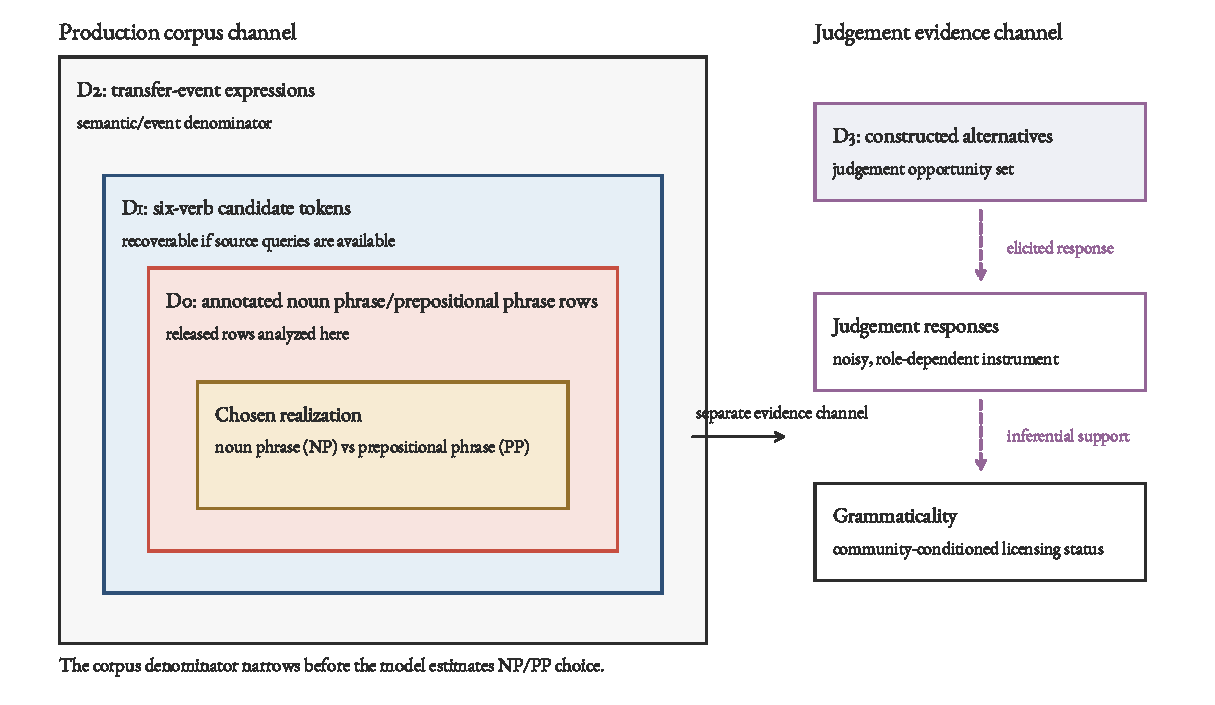
\includegraphics[width=\linewidth]{data/derived/figures/opportunity_sets_nested.pdf}
\caption{Nested opportunity sets for the dative-alternation evidence. The
released corpus rows estimate realization choice inside the annotated noun
phrase/prepositional phrase denominator. Broader transfer-event and judgement
opportunity sets would answer different questions about grammaticality.}
\label{fig:opportunity-sets}
\end{figure}

Production data can support claims about grammaticality only through an
explicit bridge from attested choices to possible alternatives. Figure
\ref{fig:opportunity-sets} marks where that bridge would have to be built.

The dative alternation makes the bridge visible. A low-probability double-object
realization may be grammatical but dispreferred under the observed predictors.
A prepositional realization may be likely because the theme is short and the
recipient is long. A form may be absent because the corpus lacks the relevant
verb, register, or discourse setting.

No amount of additional production data closes this gap. A production model
estimates choice among realizations that occurred, and it's silent by
construction about realizations that are grammatical but unattested, or
grammatical outside the sampled frame. More tokens enlarge the attested region
without ever reaching the unattested-but-grammatical one. The boundary between
production probability and grammatical possibility isn't a defect of
\texttt{languageR::dative} or BNC2014; it's a general constraint on what usage
frequency can show about grammar.

In one sense this restates a familiar point: performance data underdetermine
competence, and no finite corpus fixes the grammar
\citep{chomsky1965,Miller1963}. What the dative case adds is a measurable,
channel-specific version of that boundary. The opportunity set says which cells
a production channel can and can't reach, so the gap stops being a slogan and
becomes a property of a stated dataset and design, open to the same kind of
modelling the rest of the paper uses.

The current analyses therefore license a cautious claim. Bresnan et al.'s
production-conditioning profile is durable and partly transportable. That
supports the idea that corpus probabilities can reveal structure that informal
judgements miss. It does not make production probability identical to
grammaticality. What the durable, transportable profile does buy is prediction:
it forecasts realization for unseen tokens within its scope of verbs, registers,
and varieties, and it marks the low-probability cells where grammaticality has to
be settled through another channel.
